\section{Justification for \maf1}
\label{sec:justific}

In the following sections, we verify and justify the utility of \maf1 while also offering a comparison with popular alternatives such as \mif1, \bleu, \chrf{1}, and BLEURT.\footnote{\bleu\ and \chrf1 scores reported in this work are computed with \textsc{SacreBleu}; see the Appendix for details.
% details to put in appendix
%library with signature \texttt{\small BLEU+case.mixed+lang.<xx>-<yy>+numrefs.1 +smooth.exp+tok.<TOK>+version.1.4.13}, where \texttt{<TOK>} is \texttt{zh} for Chinese, and \texttt{13a} for all other languages. 
%\maf1 and \mif1 use the same tokenizer as \bleu.
%\chrf1 is also obtained using \textsc{SacreBleu} and has signature \texttt{\small chrF1+lang.<xx>-<yy>+numchars.6+space.false +version.1.4.13}.
BLEURT scores are from the \textit{base} model \citep{sellam-etal-2020-bleurt}. We consider two varieties of averaging to obtain a corpus-level metric from the segment-level BLEURT: mean and median of segment-level scores per corpus.
}
% Since BLEURT is a segment-level measure, we consider both \blrtmn\ and \blrtmd, which are mean and median of segment-level scores, as its corpus-level measures. \wy{moved forward to section 3}
We use Kendall's rank correlation coefficient, $\tau$, to compute the association between metrics and human judgments.
%, as $\tau$ is robust to outliers than Pearson $r$ \cite{croux2010robust-correlation}. 
%The correlation values and their p-values are computed using \texttt{scipy.stats} package \cite{2020SciPy-NMeth}. 
Correlations with p-values smaller than $\alpha=0.05$ are considered to be statistically significant.


% \subsection{Data-to-Text: WebNLG}
% \label{sec:webnlg}

% \begin{table*}[ht]
%     \footnotesize
%     \centering
%     \begin{tabular}{lrrr||rrr}
% & \multicolumn{3}{c}{ Kendall $\tau$ } & \multicolumn{3}{c}{ Pearson $r$ } \\
% Name & Fluency & Grammar & Semantics & Fluency & Grammar & Semantics \\ \hline\hline
% \bleu\  & \insig.444 & \insig.444 & \insig.500 & .788    & .836     & .780 \\
% \chrf1 & \insig.278 & \insig.278 & .778      & .742     & .803      & .889 \\
% \maf1  & \insig.222 & \insig.222 & .722     & \insig.575 & \insig.654 & .880 \\
% \mif1  & \insig.333 & \insig.333 & .611       & .752     & .814      & .871 \\ \hline
% \blrtmn & \insig.444 & \insig.444 & .833  & .808     & .854      & .922 \\
% \blrtmd & .611 & .611          & .667   & .856     & .895      & .866 \\
% \end{tabular}
%     \caption{WebNLG data-to-text task: Agreement between system-level metric scores and human judgments of fluency, grammar, and semantics. Pearson $r$ values are reported in addition to Kendall $\tau$ as many $\tau$ values are \textit{not} significant, indicated by \insig{}, at $\alpha=0.05$ (sample size is small).}
%     \label{tab:webnlg-kendall}
% \end{table*}

% In this section, we use the 2017 WebNLG Challenge dataset \cite{gardent2017webNLG-corpus, shimorina2018webnlg-human-eval}~\footnote{\myurl{https://gitlab.com/webnlg/webnlg-human-evaluation}} to analyze the differences between micro- and macro- averaging. 
% WebNLG is a task of generating English text for sets of triples extracted from DBPedia.
% Human annotations are available to a sample of 223 records each from nine NLG systems.
% %The quality of generated sentences is judged along three linguistic aspects: fluency, grammar, and semantics.\footnote{We treat semantics as semantic adequacy.}
% The human judgments provided as three linguistic aspects -- fluency, grammar, and semantics -- enable us to do a fine grained analysis of metrics.
% We use Kendall's $\tau$ and Pearson $r$ to assess agreement of system-level \bleu, \maf1, \mif1, \chrf1, \blrtmn, and \blrtmd\ that are reported in Table~\ref{tab:webnlg-kendall}.

% As seen in Table~\ref{tab:webnlg-kendall}, the metrics exhibit much variance in agreements with fluency, grammar and semantics.  
% For instance, \blrtmd\ is the best indicator of fluency and grammar, however \blrtmn\ scores the best on semantics. 
% BLEURT, being a \textit{model-based} measure that is directly trained on human judgments, scores relatively higher than others (though the decision of whether to use mean or median is unsettled).
% Considering \bleu\ as a baseline, and excluding the trained BLEURT measures, we see that \chrf1 scores high on semantics but poorly on fluency and grammar compared to \bleu.
% Not surprisingly, both \mif1 and \maf1, which rely solely on unigrams, are poor indicators of fluency and grammar compared to \bleu, however \maf1 is clearly a better indicator of semantics than \bleu. 
% The discrepancy between \mif1 and \maf1 regarding their agreement with fluency, grammar, and semantics is expected: micro averaging pays more attention to function words (as they are frequent types) that contribute to fluency and grammar where as macro-averaging pays relatively more attention to the content words that contribute to semantic adequacy. 
% %\mableu, by extending \maf1 with higher order n-grams, is found to have a good agreement with semantic adequacy while a better agreement in fluency and grammar than \maf1.

% The take away from this analysis is as follows: \maf1 is a strong indicators of semantic adequacy, however, it is a poor indicator of fluency. We recommend using either \maf1 or \chrf1 when semantic adequacy and not fluency is a desired goal.
% Caveat: WebNLG is a small dataset, and English only. 
% In the next section, we use larger datasets from tens of languages.


\subsection{Data-to-Text: WebNLG}
\label{sec:webnlg}


\begin{table}[ht]
    \footnotesize
    \centering
    \begin{tabular}{lrr}
%& \multicolumn{2}{c}{ Kendall $\tau$ }\\
Name & Fluency \& Grammar & Semantics \\ \hline\hline
\bleu\  & \insig.444 & \insig.500 \\
\chrf1 & \insig.278    & .778   \\
\maf1  & \insig.222    & .722   \\
\mif1  & \insig.333    & .611   \\ \hline
\blrtmn & \insig.444   & .833   \\
\blrtmd & .611  & .667   \\
\end{tabular}
    \caption{\small WebNLG data-to-text task: Kendall's $\tau$ between system-level MT metric scores and human judgments.
    Fluency and grammar are correlated identically by all metrics.
    Values that are \textit{not} significant at $\alpha=0.05$ are indicated by \insig{}.}
    \label{tab:webnlg-kendall}
\end{table}


We use the 2017 WebNLG Challenge dataset \cite{gardent2017webNLG-corpus, shimorina2018webnlg-human-eval}\footnote{\myurl{https://gitlab.com/webnlg/webnlg-human-evaluation}} to analyze the differences between micro- and macro- averaging. 
WebNLG is a task of generating English text for sets of triples extracted from DBPedia.
Human annotations are available for a sample of 223 records each from nine NLG systems.
%The quality of generated sentences is judged along three linguistic aspects: fluency, grammar, and semantics.\footnote{We treat semantics as semantic adequacy.}
The human judgments provided have three linguistic aspects---fluency, grammar, and semantics\footnote{Fluency and grammar, which are elicited with nearly identical directions \cite{gardent2017webNLG-corpus}, are identically correlated.}---which enable us to perform a fine grained analysis of our metrics.
We compute Kendall's $\tau$ between metrics and human judgments, which are reported in Table~\ref{tab:webnlg-kendall}.

As seen in Table~\ref{tab:webnlg-kendall}, the metrics exhibit much variance in agreements with human judgments. %Fluency and grammar display same correlations and hence are com  
For instance, \blrtmd\ is the best indicator of fluency and grammar, however \blrtmn\ is best on semantics. 
BLEURT, being a \textit{model-based} measure that is directly trained on human judgments, scores relatively higher than others.
Considering the model-free metrics, \chrf1 does well on semantics but poorly on fluency and grammar compared to \bleu.
Not surprisingly, both \mif1 and \maf1, which rely solely on unigrams, are poor indicators of fluency and grammar compared to \bleu, however \maf1 is clearly a better indicator of semantics than \bleu. 
The discrepancy between \mif1 and \maf1 regarding their agreement with fluency, grammar, and semantics is expected: micro-averaging pays more attention to function words (as they are frequent types) that contribute to fluency and grammar whereas macro-averaging pays relatively more attention to the content words that contribute to semantic adequacy. 
%\mableu, by extending \maf1 with higher order n-grams, is found to have a good agreement with semantic adequacy while a better agreement in fluency and grammar than \maf1.

The take away from this analysis is as follows: \maf1 is a strong indicator of semantic adequacy, however, it is a poor indicator of fluency. We recommend using either \maf1 or \chrf1 when semantic adequacy and not fluency is a desired goal.
%Caveat: WebNLG is a small dataset, and English only. 
%In the next section, we use larger datasets from tens of languages.



\subsection{Machine Translation: WMT Metrics}
\label{sec:wmt-metrics}

\begin{table*}[ht!]
    %\footnotesize
    \small
    \centering
    
\begin{tabular}{r r l r r r r r }
Year & Pairs  & & $\star$\bleu\ & \bleu\ & \maf1 & \mif1 & \chrf1 \\ \hline\hline
\multirow{3}{*}{ 2019 } 
    & \multirow{3}{*}{18}
     & Mean   & .751 & .771 & .821 & .818 & .841  \\ 
   & & Median & .782 & .752 & .844 & .844 & .875  \\
   & & Wins   &     3 &     3 &  \textbf{6}    &     3 &   5 \\ \hline
  %& SD     & 0.124 & 0.101 & 0.112 & 0.093 & 0.095 \\ \\
\multirow{3}{*}{ 2018 } 
  & \multirow{3}{*}{14}
   & Mean   & .858 & .857 & .875 & .873 & .902  \\ 
  & & Median & .868 & .868 & .901 & .879 & .919  \\
  & & Wins    &  1  &  2 & 3 &  2 &  \textbf{6}\\ \hline  
  %& SD     & 0.077 & 0.080 & 0.087 & 0.062 & 0.052  \\ \hline  
\multirow{3}{*}{ 2017 }
   & \multirow{3}{*}{13}
    & Mean   & .752 & .713 & .714 & .742 & .804 \\  
  & & Median & .758 & .733 & .735 & .728 & .791 \\
  & & Wins   & 5 & 4 & 2 & 2 & \textbf{6} \\
  %& SD     & 0.132 & 0.110 & 0.103 & 0.097 & 0.088 & 0.099 & 0.093 & 0.099 \\  
\end{tabular}   
\caption{WMT 2017--19 Metrics task: Mean and median Kendall's $\tau$ between MT metrics and human judgments.
%Only the mean and median $\tau$, and number of wins are reported in this table.
Correlations that are not significant at $\alpha=0.05$ are excluded from the calculation of mean, and median, and wins.
%`Wins' is number of times the achieved highest agreement with human judgments, out of total pairs in `Pairs' column.
See Appendix Tables \ref{tab:wmt19-kendall}, \ref{tab:wmt18-kendall}, and \ref{tab:wmt17-kendall} for full details.
%\maf1 and \mif1 use the same tokenizer as \bleu, whereas $\star$\bleu\ is pre-computed scores available in WMT Metrics package.
$\star$\bleu\ is pre-computed scores available in the metrics packages.
In 2018 and 2019, both \maf1 and \mif1 outperform \bleu, \maf1 outperforms \mif1.
\chrf1 has strongest mean and median agreements across the years.
Judging based on the number of wins, \maf1 has steady progress over the years, and outperforms others in 2019.
%A few outliers (that were found to be result of poor quality references) are excluded from the calculation of mean and standard deviation.
}
\label{tab:wmt-summary}
\end{table*}

In this section, we verify how well the metrics agree with human judgments using Workshop on Machine Translation (WMT) metrics task datasets for 2017--2019~\cite{WMT17-metrics,WMT18-metrics,WMT19-metrics-proceedings}.\footnote{\myurl{http://www.statmt.org/wmt19/metrics-task.html}}
%These datasets contain multiple translation directions (i.e. source$\rightarrow$target languages), and each direction contains outputs from multiple MT models along with their human judgments. 
%Unlike WebNLG, here the human judgments are a single score.
We first compute scores from each MT metric, and then calculate the correlation $\tau$ with human judgments.

As there are many language pairs and translation directions in each year, we report only the mean and median of $\tau$, and number of wins per metric for each year in Table \ref{tab:wmt-summary}. %\footnote{We report $\tau$ for individual translation directions in Tables \ref{tab:wmt19-kendall}, \ref{tab:wmt18-kendall}, and \ref{tab:wmt17-kendall} of Appendix.}
We have excluded BLEURT from comparison in this section since the BLEURT models are fine-tuned on the same datasets on which we are evaluating the other methods.\footnote{\myurl{https://github.com/google-research/bleurt}}
\chrf1 has the strongest mean and median agreement with human judgments across the years.
In 2018 and 2019, both \maf1 and \mif1 mean and median agreements outperform \bleu\, whereas in 2017 \bleu\ was better than \maf1 and \mif1.%, however \chrf1 has the strongest agreements with human judgments across the years.

%We observe that the polarity of difference between mean \maf1 and mean \mif1 has changed over the years: i.e. human agreements were better with \mif1 than \maf1 in 2017, whereas in 2019, human judgments agree better with \maf1 than \mif1.
%We observe in the recent years of WMT that \chrf1 and \maf1 outperform \bleu.
%This observation is interesting for the same reason as \maf1 outperforming \mif1.
As seen in Section~\ref{sec:webnlg}, \maf1 weighs towards semantics whereas \mif1 and \bleu\ weigh towards fluency and grammar.
This indicates that recent MT systems are mostly fluent, and adequacy is the key discriminating factor amongst them.
\bleu\ served well in the early era of statistical MT when fluency was a harder objective. 
Recent advancements in neural MT models such as Transformers \cite{vaswani2017attention} produce fluent outputs, and have brought us to an era where semantic adequacy is the focus.


% save it for the slides
%We envision that the methods such as \maf1 that emphasize the long tail be more successful in the future years, and this vision is inline with \citet{steedman-2008-last}:
%One day, either because of the demise of Moore’slaw, or simply because we have done all the easy stuff, the Long Tail will come back to haunt us.
%\textit{``One day, ... simply because we have done all the easy stuff, the Long Tail will come back to haunt us.''}

\subsection{Cross-Lingual Information Retrieval}
\label{sec:clir}
In this section, we determine correlation between MT metrics and  downstream cross-lingual information retrieval (CLIR) tasks.
CLIR is a kind of information retrieval (IR) task in which documents in one language are retrieved given queries in another~\cite{grefenstette2012CLIR}. 
A practical solution to CLIR is to translate source documents into the query language using an MT model, then use a monolingual IR system to match queries with translated documents. 
Correlation between MT and IR metrics is accomplished in the following steps: 
\begin{enumerate}[noitemsep,topsep=0pt]
 \item Build a set of MT models and measure their performance using MT metrics.
 \item Using each MT model in the set, translate all source documents to the target language, build an IR model, and measure IR performance on translated documents.
 \item For each MT metric, find the correlation between the set of MT scores and their corresponding set of IR scores.
 The MT metric that has a stronger correlation with the IR metric(s) is more useful than the ones with weaker correlations.
\item Repeat the above steps on many languages to verify the generalizability of findings.
\end{enumerate}

%\begin{figure}[ht]
%\centering
%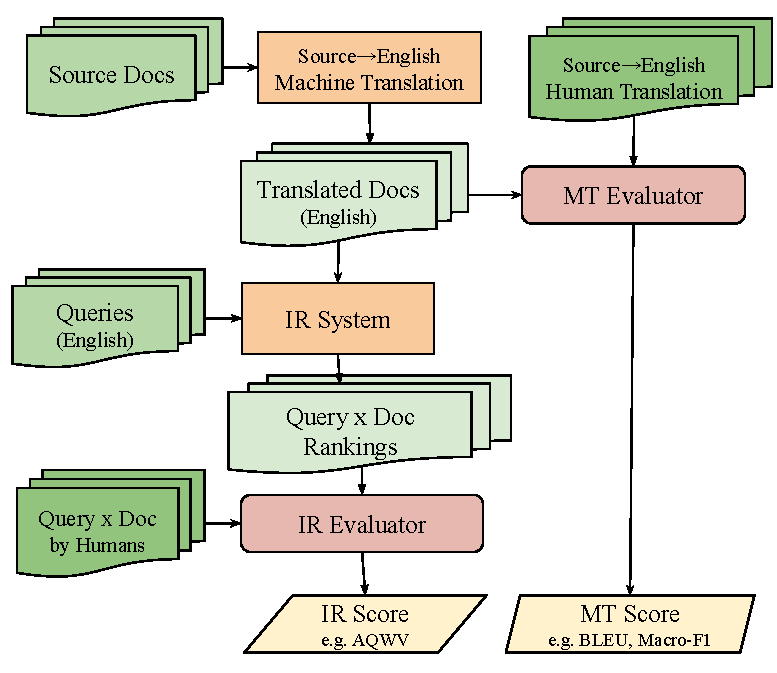
\includegraphics[width=0.9\linewidth,trim={0cm 0 0cm 0},clip]{img/CLIR-Pipe.pdf}
% to modify, goto https://docs.google.com/drawings/d/1ZrukLOtH3fQPyl9SkLWqrUqsbrSofDlSXC1tFwpYs2E/edit 
%\caption{Cross-lingual Information Retrieval system}
%\label{fig:clir-pipe}
%\end{figure}

An essential resource of this analysis is a dataset with human annotations for computing MT and IR performances.
%Specifically, this analysis requires datasets that have documents in source language and queries in target language,  along with the human translation of documents to calculate scores from MT measures, and human judgments of query to document relation to calculate IR performance.
%In addition, such datasets for a diverse set of languages are desired to verify the generalizabilty of findings.
%IARPA's Machine Translation for English Retrieval of Information in Any Language (MATERIAL) program\footnote{\myurl{https://www.iarpa.gov/index.php/research-programs/material/material-baa}} and made such datasets available, however only to its participants. 
We conduct experiments on two datasets: firstly, on data from the 2020 workshop on \textit{Cross-Language Search and Summarization of Text and Speech} (CLSSTS) \cite{zavorin-etal-2020-corpora}, and secondly, on data originally from Europarl, prepared by \citet{lignos-etal-2019-MT-IR} (Europarl).

%he restricted-access MATERIAL datasets using the systems submitted by MATERIAL performers where high-quality human judgments are available, and secondly, on publicly available datasets prepared by with a few assumptions on query-relevance judgments.

\subsubsection{CLSSTS Datasets}
\label{sec:material}

\begin{table*}[ht]
    \footnotesize
    \begin{tabular}{l l l r r r r r r }
 & Domain & IR Score & \bleu\ & \maf1 & \mif1 & \chrf1 & \blrtmn & \blrtmd \\\hline\hline

\multirow{4}{*}{LT-EN} 
& \multirow{2}{*}{In} 
  & AQWV & .429 & \insig.363 & \textbf{.508} & \insig.385 & .451  & .420 \\
& & MAP  & .495  & .429      & \textbf{.575} & .451       & .473  & .486 \\
& \multirow{2}{*}{In+Ext}
   & AQWV & \insig.345 & \textbf{.527} & .491  & .491 & .491 & .477 \\
&  & MAP  & \insig.273 & \insig\textbf{.455} & \insig.418 & \insig.418 & \insig.418 & \insig.404 \\\hline
\multirow{4}{*}{PS-EN}
  & \multirow{2}{*}{In} 
    & AQWV  & .559 & \textbf{.653} & .574 & .581 & .584 & .581  \\
  & & MAP   & .493 & \textbf{.632} & .487 & .494 & .558 & .554 \\
  & \multirow{2}{*}{In+Ext}
    & AQWV   & .589 & \textbf{.682} & .593 & .583 & .581 & .571 \\
  & & MAP    & .519 & \textbf{.637} & .523 & .482 & .536 & .526 \\\hline
\multirow{4}{*}{BG-EN}
 & \multirow{2}{*}{In} 
    & AQWV   & \insig.455 & \textbf{.550}   & .527  & \insig.382 & \insig.418  & .418 \\ 
 &  & MAP    &  .491      &  \textbf{.661}  & .564  &  .491       & .527       & .527 \\ 
 & \multirow{2}{*}{In+ext}
    & AQWV   & \insig.257 & \textbf{.500}       & \insig.330 & \insig.404 & \insig.367 & \insig.367 \\
 &  & MAP   & \insig.183 & \insig\textbf{.426} & \insig.257 & \insig.330 & \insig.294 & \insig.294 
\end{tabular} 
\caption{CLSSTS CLIR task: Kendall's $\tau$ between IR and MT metrics under study.
The rows with Domain=In are where MT and IR scores are computed on the same set of documents, whereas Domain=In+Ext are where IR scores are computed on a larger set of documents that is a superset of segments on which MT scores are computed.
\textbf{Bold} values are the best correlations achieved in a row-wise setting; values with \insig~ are \textit{not} significant at $\alpha=0.05$.}
\label{tab:material-kendall}
\end{table*}


CLSSTS datasets contain queries in English~(EN), and documents in many source languages along with their human translations, as well as query-document relevance judgments. 
We use three source languages: Lithuanian~(LT), Pashto~(PS), and Bulgarian~(BG).
The performance of this CLIR task is evaluated using two IR measures: Actual Query Weighted Value (AQWV) and Mean Average Precision (MAP).
AQWV\footnote{\href{https://www.nist.gov/system/files/documents/2017/10/26/aqwv\_derivation.pdf}{https://www.nist.gov/system/files/documents-/2017/10/26/aqwv\_derivation.pdf}} is derived from Actual Term Weighted Value (ATWV) metric \cite{wegmann2013ATWV}. 
%, being the official metric of MATERIAL program,
% by National Institute of Standards and Technology~(NIST). 
%The nature of AQWV is such that a higher score implies better CLIR performance. 
%Since the focus of this analysis is on MT evaluation methods and not the MT systems, we treat all MT systems as blackboxes for which internal details are unnecessary; however, we clarify that the MT systems used are representative of commonly used models such as convolutional \cite{gehring2017cnn} and Transformer~\cite{vaswani2017attention} NMT models, as well as once-popular syntax-based string-to-tree statistical MT~\cite{galley-etal-2004-sbmt}.


%The high level overview of our CLIR pipeline is shown in Figure \ref{fig:clir-pipe}:
%First, documents in source language are translated to English using a set of MT models. 
%Performance of all MT models is evaluated on the same set of documents using their corresponding human translations.
%The translated documents are indexed by an IR system, and the end-to-end performance on a set of queries is evaluated using AQWV metric with the help of human created judgments.
%Our CLIR system is based on \citet{boschee-etal-2019-saral}, which is competitive in the workshop on CLSSTS-2020~\cite{clssts-2020}.
%Since the CLIR system is also treated as a blackbox, the internals of CLIR is unnecessary and beyond the scope of this work.
We use a single CLIR system \cite{boschee-etal-2019-saral} with the same IR settings for all MT models in the set, and measure Kendall's $\tau$ between MT and IR measures.
The results, in Table~\ref{tab:material-kendall}, show that \maf1 is the strongest indicator of CLIR downstream task performance in five out of six settings.
AQWV and MAP have a similar trend in agreement to the MT metrics.
\chrf1 and BLEURT, which are strong contenders when generated text is directly evaluated by humans, do not indicate CLIR task performance as well as \maf1, as CLIR tasks require faithful meaning equivalence across the language boundary, and human translators can mistake fluent output for proper translations \cite{callison-burch-etal-2007-meta}. 
%Hence, we recommend the use of \maf1 when MT output is used in downstream tasks such as IR.



\subsubsection{Europarl Datasets} %\tg{pick more informative section name?}
\label{sec:lignos-etal}

\begin{table}[ht]
    \footnotesize
    \centering
\begin{tabular}{l@{\hspace{1mm}} r@{\hspace{1mm}} r@{\hspace{1mm}} r@{\hspace{1mm}} r@{\hspace{1.2mm}} r@{\hspace{1.2mm}} r}
 & \bleu\ & \maf1 & \mif1 & \chrf1 & $\overline{\text{BT}}$ & $\widetilde{\text{BT}}$ \\ \hline\hline
\multirow{1}{*}{ CS-EN } 
%& MAP  & \textbf{.950} & .933 & \textbf{.950} & \textbf{.950} & .900 & .933 \\
%& MAP  & \textbf{.95} & .93 & \textbf{.95} & \textbf{.95} & .90 & .93 \\
 & .850 & .867 & .850 & .850 & \textbf{.900} & .867 \\ 
%& RBO  & .85 & .87 & .85 & .85 & \textbf{.90} & .87 \\ \hline
\multirow{1}{*}{ DE-EN } 
%& MAP  & .862 & .895 & .862 & .874 & \textbf{.912} & .895 \\
%& MAP  & .86 & .90 & .86 & .87 & .91 & .90 \\
  & .900 & .900 & .900 & .912 & \textbf{.917} & .900 \\
%& RBO  & .90 & .90 & .90 & .91 & .92 & .90 \\
\end{tabular}  
\caption{Europarl CLIR task: Kendall's $\tau$ between MT metrics and RBO. $\overline{\text{BT}}$ and $\widetilde{\text{BT}}$ are short for \blrtmn\ and \blrtmd. All correlations are significant at $\alpha=0.05$.}
\label{tab:lignos-mtir-kendall} 
\end{table}


We perform a similar analysis to Section \ref{sec:material} but on another cross-lingual task set up by \citet{lignos-etal-2019-MT-IR} for Czech $\rightarrow$ English (CS-EN) and German $\rightarrow$ English (DE-EN), using publicly available data from the Europarl v7 corpus~\cite{koehn2005europarl}. 
%The IR model used is a term-based approach based on Okapi-BM25~\cite{jones2000probabilistic}.
%This task uses publicly available datasets; specifically documents from the Europarl v7 corpus~\cite{koehn2005europarl} for English, Czech, and German. 
This task differs from the CLSSTS task (Section \ref{sec:material}) in several ways.
Firstly, MT metrics are computed on test sets from the news domain, whereas IR metrics are from the Europarl domain. The domains are thus intentionally mismatched between MT and IR tests.
Secondly, since there are no queries specifically created for the Europarl domain, GOV2 TREC topics 701–850 are used as domain-relevant English queries.
And lastly, since there are no query-document relevance human judgments for the chosen query and document sets, the documents retrieved by BM25~\cite{jones2000probabilistic} on the English set for each query are treated as relevant documents for computing the performance of the CS-EN and DE-EN CLIR setup. 
As a result, IR metrics that rely on boolean query-document relevance judgments as ground truth are less informative, and we use Rank-Based Overlap (RBO; $p=0.98$) \cite{webber2010RBO} as our IR metric.

We perform our analysis on the same experiments as \citet{lignos-etal-2019-MT-IR}.\footnote{\myurl{https://github.com/ConstantineLignos/mt-clir-emnlp-2019}}
NMT models for CS-EN and DE-EN translation are trained using a convolutional NMT architecture \cite{gehring2017cnn} implemented in the FAIRSeq~\cite{ott2019fairseq} toolkit.
For each of CS-EN and DE-EN, a total of 16 NMT models that are based on different quantities of training data and BPE hyperparameter values are used.
%We report two IR metrics, namely: Rank-Based Overlap (RBO; $p=0.98$) \cite{webber2010RBO}, and Mean Average Precision (MAP), and their correlations with MT metrics.
The results in Table~\ref{tab:lignos-mtir-kendall} show that BLEURT has highest correlation in both cases.
Apart from the trained \blrtmd\ metric, \maf1 scores higher than the others on CS-EN, and is competitive on CS-EN. \maf1 is not the metric with highest IR task correlation in this setting, unlike in Section \ref{sec:material}, however it is competitive with \bleu\ and \chrf1, and thus a safe choice as a downstream task performance indicator. 

